\section{Methods: A Characterization Framework}
\label{sec:methods}

To understand the spatial and functional contribution of decoder computation, we establish a controlled observation framework (Figure \ref{fig:framework}). We evaluate matched pairs of full and efficient decoders as experimental probes under two complementary regimes: (i) \textit{end-to-end model comparison} across independently trained networks to assess real-world generalization, and (ii) \textit{decoder-isolated attribution analysis} using frozen shared encoders to isolate decoder capacity interventions.

\begin{figure*}[t]
\centering
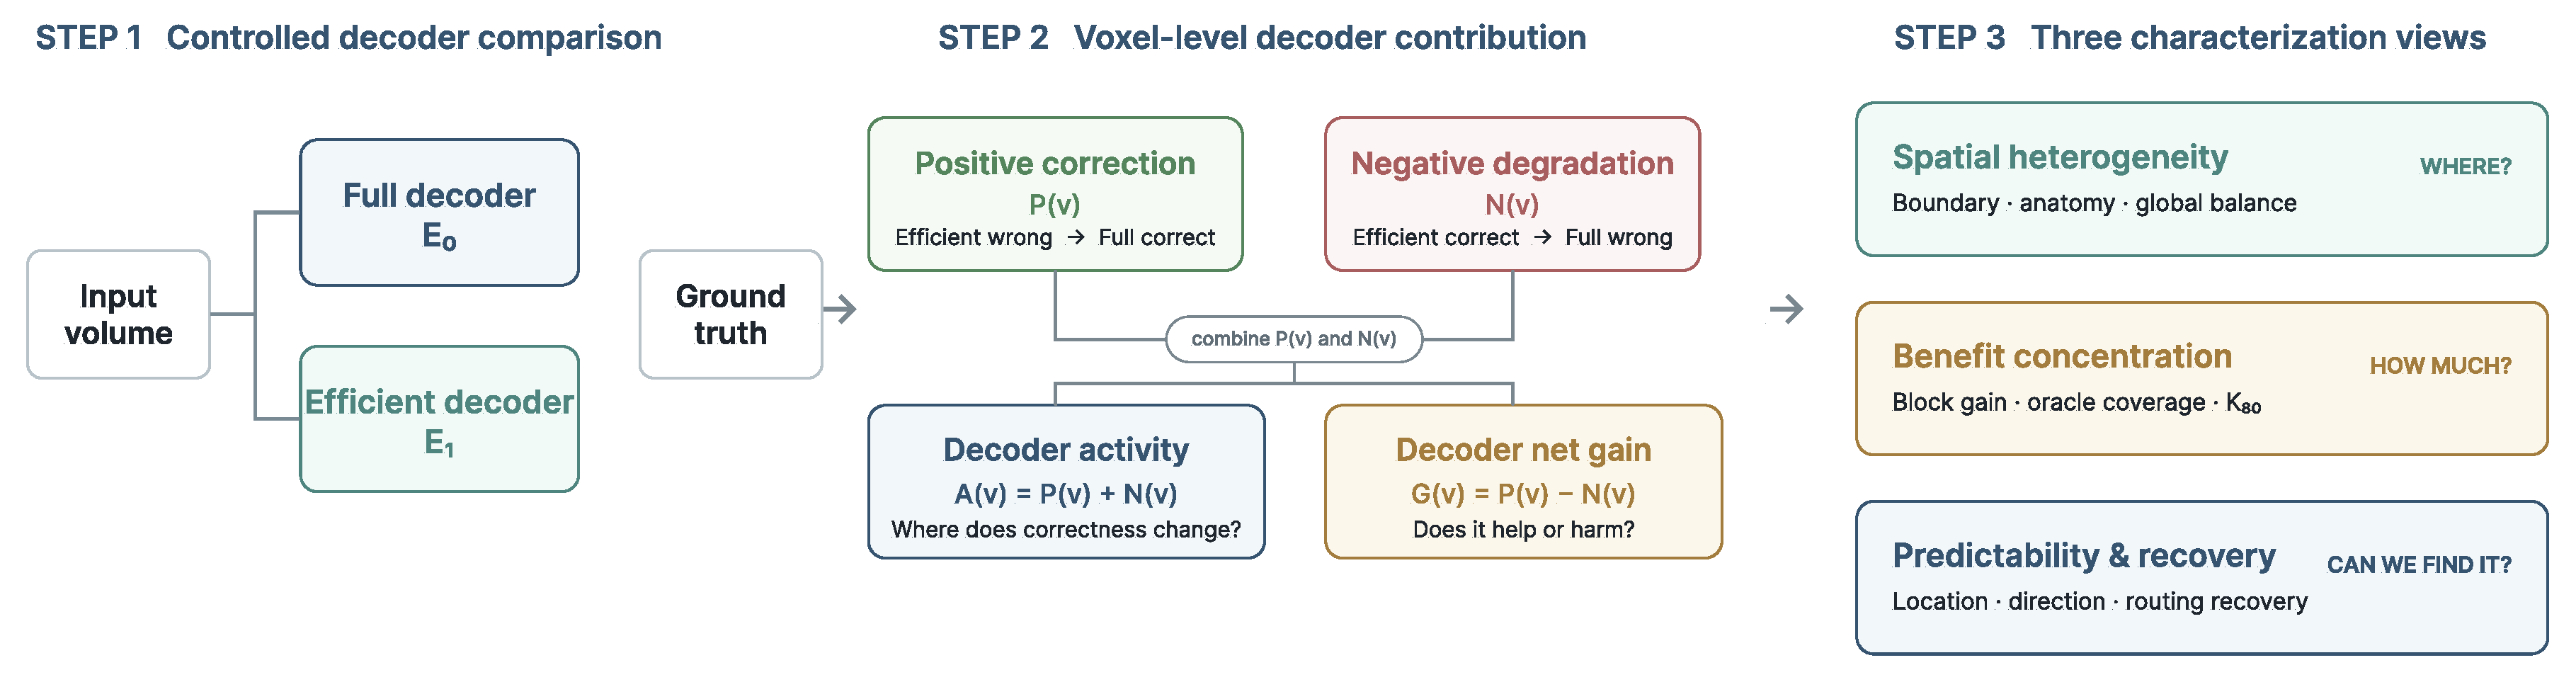
\includegraphics[width=0.98\textwidth]{figures/figure1_framework}
\caption{Overview of the decoder-computation characterization framework. Step 1 (Controlled Decoder Comparisons): Full and efficient decoder pairs are evaluated under two complementary regimes (independently trained end-to-end pairs for cross-architecture consistency, and frozen shared-encoder factorials for decoder-isolated causal attribution). Step 2 (Voxel Activity and Net Gain): Voxel-level corrections and degradations establish the fundamental dichotomy between Decoder Activity (where the decoder acts) and Net Gain (where it helps). Step 3 (Three Characterization Axes): Probes spatial heterogeneity, benefit concentration, and predictability. Step 4 (Design Implications): Translates empirical insights into evidence-backed directions for adaptive decoder design.}
\label{fig:framework}
\end{figure*}

\subsection{Controlled Decoder Comparison}
Let $v$ denote a voxel within a 3D medical image volume $V$. We compare two decoder configurations:
\begin{itemize}
    \item \textbf{Full Decoder ($E_0$)}: The standard dense, multi-stage high-resolution decoder of the respective backbone architecture.
    \item \textbf{Efficient Decoder ($E_1$)}: A parameter-matched efficient decoder following the EffiDec3D specification \cite{effidec3d}, utilizing channel reduction and stage removal with concatenation skip aggregation.
\end{itemize}
Let $y(v)$ be the ground truth label, $\hat{y}_f(v)$ be the prediction from the full decoder, and $\hat{y}_e(v)$ be the prediction from the efficient decoder. Interventions occur strictly within the decoder pathway (upsampling, skip fusion, and refinement).

\begin{table*}[t]
\centering
\caption{Overview of characterization objectives and evaluation measures.}
\label{tab:framework_summary}
\small
\begin{tabular*}{\textwidth}{@{\extracolsep{\fill}}lll}
\toprule
\textbf{Analysis Objective} & \textbf{Evaluation Measure} & \textbf{Question Answered} \\
\midrule
Spatial effect & Activity $A(v)$ & Where does additional decoder computation change predictions? \\
Directional effect & Net Gain $G(v)$ & Where does the decoder improve correctness overall? \\
Concentration & Oracle $K_{80}$ & How spatially concentrated is positive net gain? \\
Activity predictability & Location AUROC & Can cheap signals detect where the decoder acts? \\
Gain predictability & Direction AUROC & Can cheap signals distinguish beneficial from harmful changes? \\
Practical recovery & Routing Gain & Does selective execution improve segmentation metrics? \\
\bottomrule
\end{tabular*}
\end{table*}

\subsection{Decoder-Induced Corrections and Degradations}
Comparing predictions between the efficient and full decoders at each voxel yields three possible outcomes: the full decoder corrects an error, introduces an error, or leaves prediction correctness unchanged (Figure \ref{fig:motivation}; see Supplementary Figures S1 and S2 for SwinUNETR and MedNeXt-M-K3 qualitative visualizations):
\begin{itemize}
    \item \textbf{Positive Correction ($P(v)$)}: $P(v) = 1[\hat{y}_e(v) \neq y(v) \wedge \hat{y}_f(v) = y(v)]$.
    \item \textbf{Negative Degradation ($N(v)$)}: $N(v) = 1[\hat{y}_e(v) = y(v) \wedge \hat{y}_f(v) \neq y(v)]$.
\end{itemize}
We define two fundamental analytical quantities:
\begin{itemize}
    \item \textbf{Decoder Activity ($A(v) = P(v) + N(v)$)}: Indicates where additional decoder capacity alters prediction correctness, regardless of direction.
    \item \textbf{Decoder Net Gain ($G(v) = P(v) - N(v)$)}: Distinguishes beneficial corrections from harmful degradations.
\end{itemize}
\textit{Decoder activity measures where the decoder acts, whereas decoder gain measures whether those changes are beneficial or harmful.}

\begin{figure*}[t]
\centering

\includegraphics[width=0.9\textwidth]{figures/obs-uxnet-concat/figure1_motivation}
\caption{Qualitative illustration of decoder activity and directional gain (3D UX-Net on BTCV CT multi-organ dataset). While the full decoder corrects certain errors of the efficient baseline (positive flips), it also alters previously correct predictions (negative flips) near high-entropy organ boundaries, demonstrating non-uniform spatial contribution (see Supplementary Figures S1 and S2 for SwinUNETR and MedNeXt-M-K3).}
\label{fig:motivation}
\end{figure*}

\subsection{Spatial Characterization of Decoder Effects}
We analyze Activity $A(v)$ and Net Gain $G(v)$ across two spatial dimensions:
\begin{enumerate}
    \item \textbf{Boundary-Distance Stratification}: Distance to the nearest organ boundary using a multi-class union foreground mask $\bigcup_{c} (y(v)=c \cup \hat{y}_e(v)=c \cup \hat{y}_f(v)=c)$ \cite{taha2015metrics}.
    \item \textbf{Anatomical Structure Breakdown}: Aggregated $A(v)$ and $G(v)$ across individual organ structures.
\end{enumerate}

\subsection{Spatial Concentration and Oracle Opportunity}
We partition the 3D volume into spatial sub-blocks $b_r$ and compute block net gain:
\begin{equation}
G(r) = \sum_{v \in b_r} G(v)
\end{equation}
Sorting blocks by $G(r)$, the fraction of positive gain recovered by the top $k\%$ of blocks is defined by the coverage curve:
\begin{equation}
Coverage(k) = \frac{\sum_{r=1}^{k\% \cdot |B|} \max(G(r), 0)}{\sum_{r=1}^{|B|} \max(G(r), 0)}
\end{equation}
We record $K_{80}$, defined as the smallest fraction of spatial blocks required by a perfect selector to recover 80\% of the total positive decoder gain. A selective hybrid prediction $\hat{y}_k(v)$ executes the full decoder on selected blocks $S_k$ and the efficient baseline elsewhere:
\begin{equation}
\hat{y}_k(v) = \begin{cases}
\hat{y}_f(v), & \text{if } v \in S_k \\
\hat{y}_e(v), & \text{otherwise}
\end{cases}
\end{equation}

\subsection{Predictability and Practical Routing Gain}
We compute predictive Shannon entropy $H(v)$ from the efficient baseline outputs \cite{shannon1948mathematical,gal2016dropout}:
\begin{equation}
H(v) = -\sum_{c=1}^{C} p_c(v) \log p_c(v)
\end{equation}
where $p_c(v)$ represents the softmax probability for class $c$ at voxel $v$. Using $H(v)$, we evaluate three predictability measures:
\begin{enumerate}
    \item \textbf{Location AUROC}: Discrimination of active blocks ($A(r) > 0$) vs. inactive blocks ($A(r) = 0$) \cite{hendrycks2017baseline}.
    \item \textbf{Direction AUROC}: Discrimination of net positive blocks ($G(r) > 0$) vs. net negative blocks ($G(r) < 0$) \cite{cmig2025quality}.
    \item \textbf{Practical Routing Gain}: Segmentation metric recovery (Dice/HD95) achieved by entropy-guided selection over the efficient baseline $E_1$, compared against a random selection baseline under identical spatial budgets.
\end{enumerate}
